\section{Messung des Stillstandsdrehmomentes}

\subsection{Beschreibung}

Im dritten Versuch soll die Konstante $k_e$ bestimmt werden. Diese
hängt proportional mit der Spannung $U_i$ und der Winkelgeschwindigkeit
$\omega$ zusammen.

\begin{equation} \label{eq131}
    \begin{split}
        u_a(t)=k_e \cdot \omega (t)
    \end{split}
\end{equation}

Gegeben ist in dieser Aufgabe eine Matrix mit den Spannungswerten von
$U_a$ und den Inkrementen des Rotaryencoders pro $\mathrm{ms}$.

\begin{equation} \label{eq132}
    \begin{split}
        Y& \quad \text{in} \quad \left[\frac{\mathrm{Ink}}{\mathrm{ms}}\right]\\
        X& \quad \text{in} \quad [V]
    \end{split}
\end{equation}

Desweiteren hat der Inkrementalgeber eine Pulszahl von $P_z=\frac{2000}{2\pi} \mathrm{\frac{pulse}{rad}}$
und wird in Vierfachauswertung $\alpha=4$ betrieben.

\begin{equation} \label{eq133}
    \begin{split}
        \lambda = \frac{P_z}{\alpha} = \frac{250}{\pi} \mathrm{\frac{Ink}{rad}}
    \end{split}
\end{equation}

Die Winkelgeschwindigkeit $\omega(t)$ ist wie folgt definiert.

\begin{equation} \label{eq134}
    \begin{split}
       \omega(t)= 2 \pi n(t)=2 \pi \frac{y(t)}{\lambda} \quad \text{in} \quad \left[\mathrm{\frac{rad}{ms}} \right]
    \end{split}
\end{equation}

Dadurch berechnet sich $ke$ nach über das Reziproke der Steigung der Funktion
multipliziert mit dem Faktor $\lambda$.

\begin{equation} \label{eq134}
    \begin{split}
    k_e = \frac{1}{m} \cdot \lambda \cdot \frac{1}{1000} = 58.801 \cdot 10^{-4} \mathrm{\frac{Vs}{rad}}
    \end{split}
\end{equation}




\subsection{Ausgabe der Lösung}
\begin{figure}[H]
 \centering
 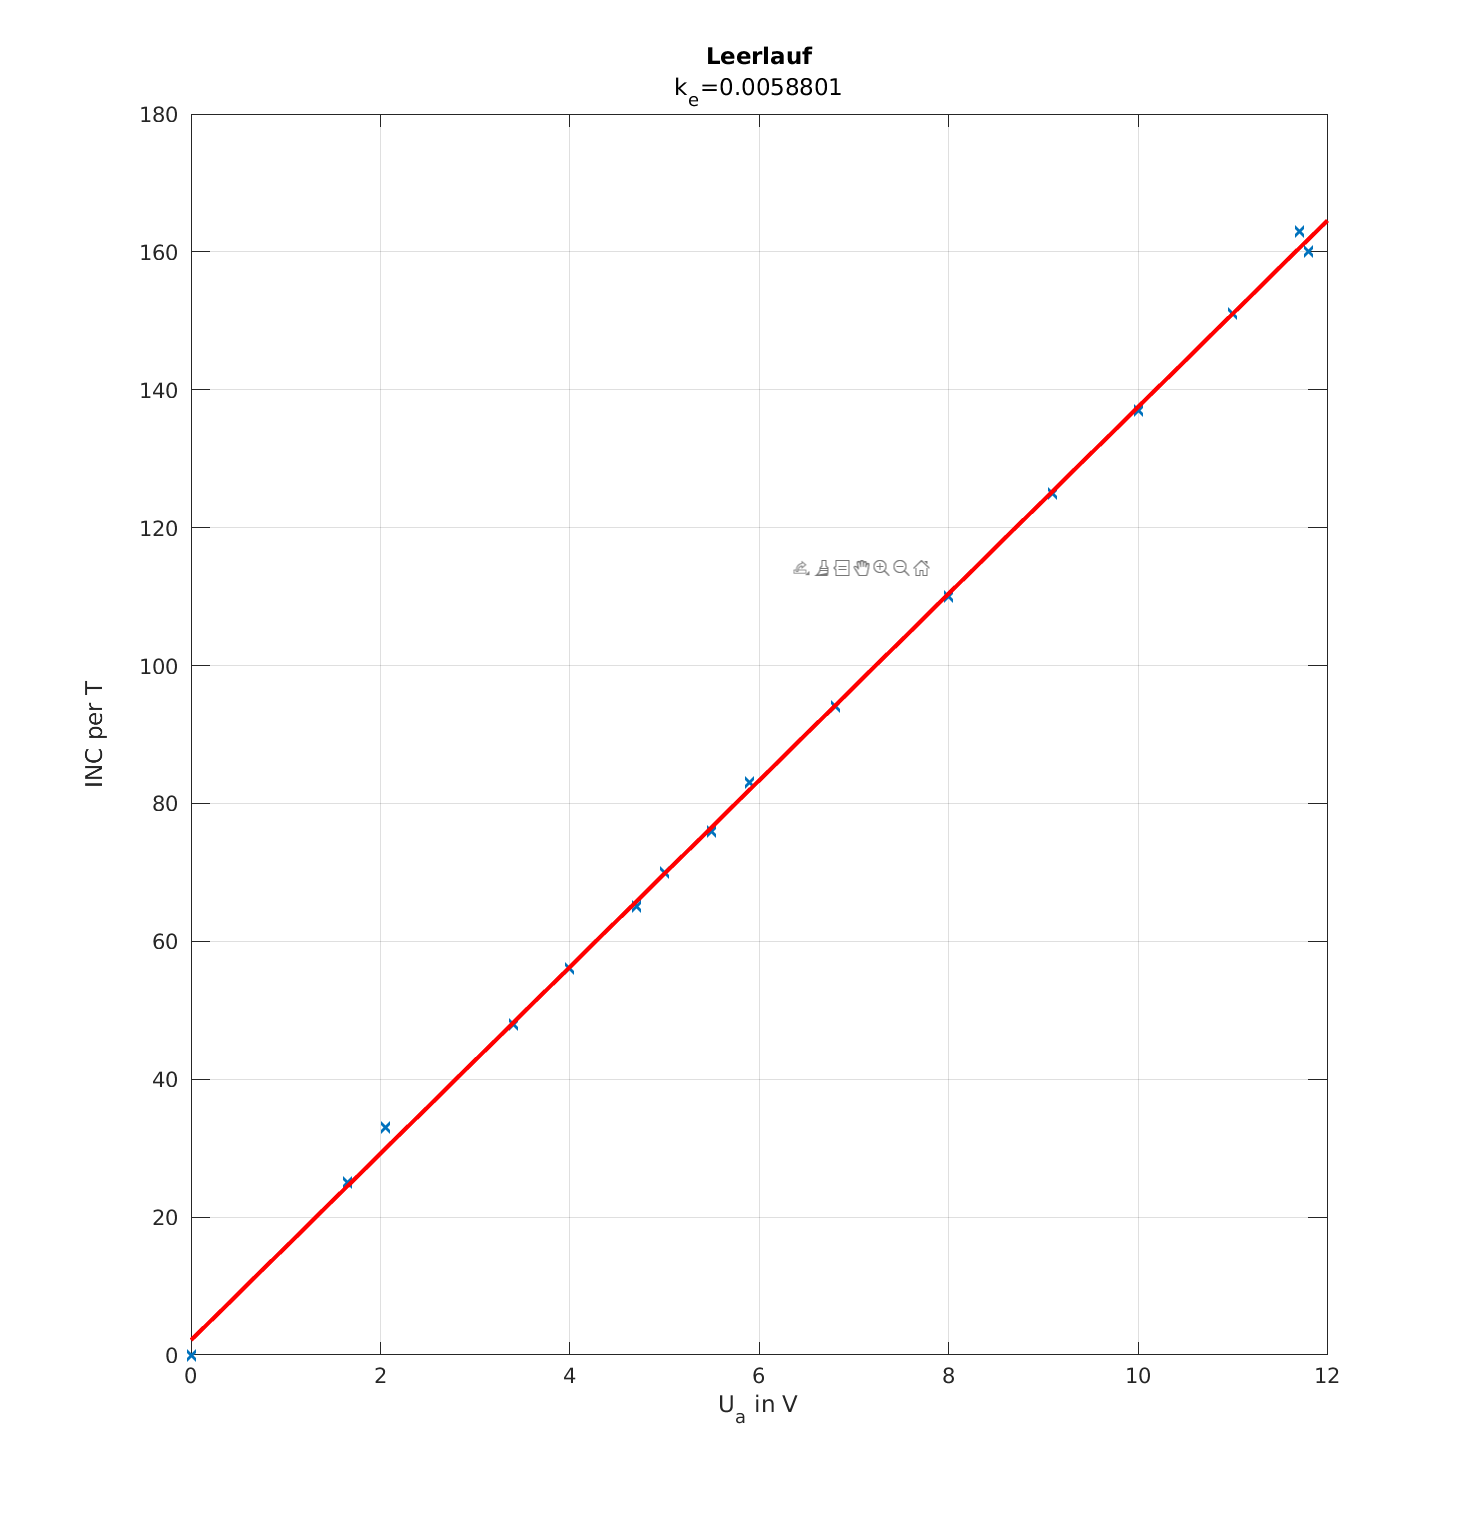
\includegraphics[width=1\textwidth]{as_labor01_3.png}
 \caption{Plot der Aufgabe 3}
 \label{fig:PlotAufgabe3}
\end{figure}

\subsection{Matlab Code}
\lstinputlisting[language=Matlab]{matlab/as_labor01_3.m}
